\documentclass[8pt]{beamer}

 \usepackage[utf8]{inputenc}                                                     
  \usetheme{Bergen}                                                               
  \usecolortheme{crane}                                                       
  %\useinnertheme{circles}                                                         
  \usepackage[english]{babel}                                                     
  \usepackage{csquotes}                                                           
  \usepackage[T1]{fontenc}                                                        
  \usepackage{booktabs}                                                           
  \usepackage{amsmath}   
  \usepackage{tikz}
  \usepackage{amssymb}
  \usepackage{amsfonts}
  \usepackage{mathrsfs}   
  \usepackage{graphicx}
  \usepackage{varioref}
  \usepackage[style=authoryear,backref=true]{biblatex}
 \usepackage[]{hyperref} 
  \graphicspath{{Graphics/}}
  \usepackage{multirow,array}
  \addbibresource{../Everything.bib}
  \usepackage{colortbl}
  \definecolor{aa}{RGB}{247, 232, 35}
  \definecolor{cc}{RGB}{29, 23, 80}    
  %\setbeamercolor{palette tertiary}{fg=aa,bg=cc}
  %\setbeamercolor{structure}{fg=cc}
  %\setbeamercolor{alerted text}{fg=red}
  
  %Information to be included in the title page:
  \title[Discrete]{AL FM Discrete}
  
  \subtitle{Fundamentals of Graph Theory}
  
  \author[]{T. Bretschneider}
  
  \date[\today]{\today}

\usepackage{comment}
\usepackage{varwidth}

\begin{document}

\frame{\titlepage}

\begin{frame}
\frametitle{Outline}
\tableofcontents

\end{frame}


\section{Introduction}

\begin{frame}{What is Graph Theory?}
	A graph has two meanings in Mathematics. 
\usetikzlibrary{shapes.geometric}
\begin{center}
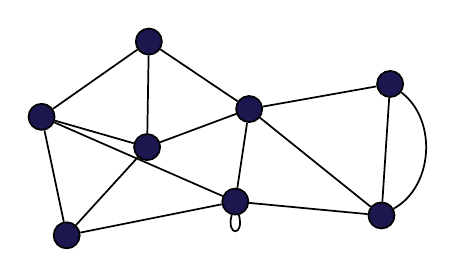
\begin{tikzpicture}[scale=0.5]
[every node/.style={inner sep=0pt,scale=0.5}]
\node (1) [circle, minimum size=6pt, fill=cc, line width=0.625pt, draw=black] at (110.0pt, -160.625pt)  {};
\node (2) [circle, minimum size=6pt, fill=cc, line width=0.625pt, draw=black] at (187.5pt, -106.25pt)  {};
\node (3) [circle, minimum size=6pt, fill=cc, line width=0.625pt, draw=black] at (260.0pt, -155.0pt)  {};
\node (4) [circle, minimum size=6pt, fill=cc, line width=0.625pt, draw=black] at (361.875pt, -136.875pt)  {};
\node (5) [circle, minimum size=6pt, fill=cc, line width=0.625pt, draw=black] at (355.625pt, -231.875pt)  {};
\node (6) [circle, minimum size=6pt, fill=cc, line width=0.625pt, draw=black] at (250.0pt, -221.875pt)  {};
\node (7) [circle, minimum size=6pt, fill=cc, line width=0.625pt, draw=black] at (186.25pt, -182.5pt)  {};
\node (8) [circle, minimum size=6pt, fill=cc, line width=0.625pt, draw=black] at (128.125pt, -246.25pt)  {};
\draw [line width=0.625, color=black] (8) to  (1);
\draw [line width=0.625, color=black] (1) to  (7);
\draw [line width=0.625, color=black] (7) to  (8);
\draw [line width=0.625, color=black] (2) to  (7);
\draw [line width=0.625, color=black] (1) to  (2);
\draw [line width=0.625, color=black] (8) to  (6);
\draw [line width=0.625, color=black] (6) to  (1);
\draw [line width=0.625, color=black] (2) to  (3);
\draw [line width=0.625, color=black] (3) to  (4);
\draw [line width=0.625, color=black] (4) to  [in=29, out=323] (5);
\draw [line width=0.625, color=black] (6) to  (5);
\draw [line width=0.625, color=black] (5) to  (4);
\draw [line width=0.625, color=black] (3) to  (5);
\draw [line width=0.625, color=black] (3) to  (6);
\draw [line width=0.625, color=black] (7) to  (3);
\draw [line width=0.625, color=black, loop below] (6) to (6);
\end{tikzpicture}
\end{center}
	% Pictures needed!!!!!	
	It can be a plot showing how two objects relate to each other. Or a representation of connections between objects. 

	\begin{alertblock}{Definition of a graph}
		A graph is made of:
		\begin{itemize}
			\item A vertex set of objects.
			\item An edge set where two vertices are connected if the edge between them is in the edge set. 
		\end{itemize}
	\end{alertblock}
	
\end{frame}

\begin{frame}{Representing Graphs}
	\begin{center}
	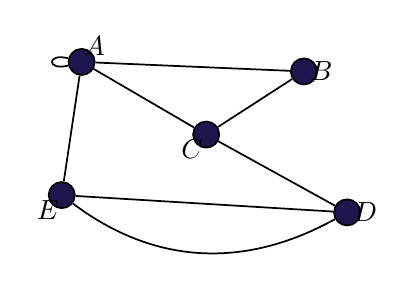
\begin{tikzpicture}[scale=0.5]
[every node/.style={inner sep=0pt}]
\node (1) [circle, minimum size=6pt, fill=cc, line width=0.625pt, draw=black] at (114.375pt, -155.0pt)  {};
\node (2) [circle, minimum size=6pt, fill=cc, line width=0.625pt, draw=black] at (275.0pt, -161.875pt)  {};
\node (3) [circle, minimum size=6pt, fill=cc, line width=0.625pt, draw=black] at (204.375pt, -207.5pt)  {};
\node (4) [circle, minimum size=6pt, fill=cc, line width=0.625pt, draw=black] at (100.0pt, -251.25pt)  {};
\node (5) [circle, minimum size=6pt, fill=cc, line width=0.625pt, draw=black] at (306.25pt, -263.75pt)  {};
\draw [line width=0.625, color=black] (1) to  (2);
\draw [line width=0.625, color=black] (1) to  (3);
\draw [line width=0.625, color=black] (3) to  (2);
\draw [line width=0.625, color=black] (5) to  (3);
\draw [line width=0.625, color=black] (5) to  (4);
\draw [line width=0.625, color=black] (4) to  [in=209, out=323] (5);
\draw [line width=0.625, color=black] (1) to  (4);
\draw [line width=0.625, color=black, loop left] (1) to (1);
\node at (123.75pt, -143.75pt) {\textcolor{black}{$A$}};
\node at (287.5pt, -161.875pt) {\textcolor{black}{$B$}};
\node at (194.375pt, -218.125pt) {\textcolor{black}{$C$}};
\node at (90.0pt, -261.875pt) {\textcolor{black}{$E$}};
\node at (319.375pt, -263.75pt) {\textcolor{black}{$D$}};
\end{tikzpicture}
\end{center}

The vertex set of this graph would be ${A,B,C,D,E}$.

And, the edge set would be  ${(A,A),(A,B),(A,C),(A,E),(B,C),(C,D),(D,E),(D,E)}$.

Rather than writing out the sets explicitly we usually prefer to represent the graph pictorially (as above) or use an adjacency matrix (as below).

\begin{center}
	\colorbox{cc!30}{
		\setlength\arrayrulewidth{0.5mm}
		\arrayrulecolor{white}
\begin{tabular}{c|ccccc}
	& $A$ & $B$ & $C$ & $D$ & $E$ \\
	\hline
	$A$ & 2 & 1 & 1 & 0 & 1 \\
	$B$ & 1 & 0 & 1 & 0 & 0 \\
	$C$ & 1 & 1 & 0 & 1 & 0 \\
	$D$ & 0 & 0 & 1 & 0 & 2 \\
	$E$ & 1 & 0 & 0 & 2 & 0 \\
\end{tabular}}
\end{center}
\begin{alertblock}{The adjacency matrix}
	\begin{itemize}
		\item Each entry represents the number of edges between the vertex corresponding to that row and column. The entry $a_{ij}$, will give the number of edges between vertex $i$ and vertex  $j$.
		\item For a graph this will always result in a triangular matrix.
		\item The loop counts as 2.
	\end{itemize}
	
\end{alertblock}
\end{frame}
\begin{frame}{Degree of a Vertex}
	\begin{alertblock}{Definition of Degree}
		The \textbf{degree} of a vertex is the number of edges that are adjacent to that vertex. Loop counts twice. 
	\end{alertblock}
	\usetikzlibrary{calc}

	\begin{center}
	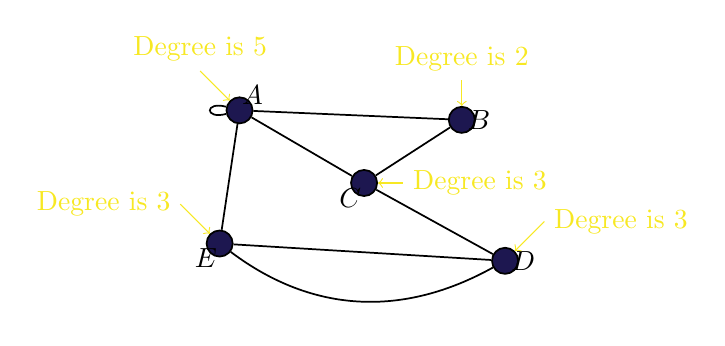
\begin{tikzpicture}[scale=0.5]
[every node/.style={inner sep=0pt}]
\node (1) [circle, minimum size=6pt, fill=cc, line width=0.625pt, draw=black] at (114.375pt, -155.0pt)  {};
\node (2) [circle, minimum size=6pt, fill=cc, line width=0.625pt, draw=black] at (275.0pt, -161.875pt)  {};
\node (3) [circle, minimum size=6pt, fill=cc, line width=0.625pt, draw=black] at (204.375pt, -207.5pt)  {};
\node (4) [circle, minimum size=6pt, fill=cc, line width=0.625pt, draw=black] at (100.0pt, -251.25pt)  {};
\node (5) [circle, minimum size=6pt, fill=cc, line width=0.625pt, draw=black] at (306.25pt, -263.75pt)  {};
\draw [line width=0.625, color=black] (1) to  (2);
\draw [line width=0.625, color=black] (1) to  (3);
\draw [line width=0.625, color=black] (3) to  (2);
\draw [line width=0.625, color=black] (5) to  (3);
\draw [line width=0.625, color=black] (5) to  (4);
\draw [line width=0.625, color=black] (4) to  [in=209, out=323] (5);
\draw [line width=0.625, color=black] (1) to  (4);
\draw [line width=0.625, color=black, loop left] (1) to (1);
\node at (123.75pt, -143.75pt) {\textcolor{black}{$A$}};
\node at (287.5pt, -161.875pt) {\textcolor{black}{$B$}};
\node at (194.375pt, -218.125pt) {\textcolor{black}{$C$}};
\node at (90.0pt, -261.875pt) {\textcolor{black}{$E$}};
\node at (319.375pt, -263.75pt) {\textcolor{black}{$D$}};
\draw [color=aa, <-] (1) --++ (-1,1) node[above] {Degree is $5$};
\draw [color=aa, <-] (2) --++ (0,1) node[above] {Degree is $2$};
\draw [color=aa, <-] (3) --++ (1,0) node[right] {Degree is $3$};
\draw [color=aa, <-] (5) --++ (1,1) node[right] {Degree is $3$};
\draw [color=aa, <-] (4) --++ (-1,1) node[left] {Degree is $3$};
\end{tikzpicture}
\end{center}

The degree can also be calculated from the adjacency matrix by adding the numbers in the corresponding row or column.

\begin{Problem}
	A graph has 5 vertices and 6 edges. Find the sum of the degrees of the vertices.

	Answer: 12
	
\end{Problem}
\end{frame}

\section{Graph types}%

\begin{frame}{Simple Graphs}
	\begin{alertblock}{Multiple edges}
		Two vertices have \textbf{multiple edges} between them if there are two or more edges between them. 
	\end{alertblock}
	\begin{alertblock}{Loop}
		A \textbf{loop} is an edge which starts and ends at the same vertex. 
	\end{alertblock}
	\begin{center}
	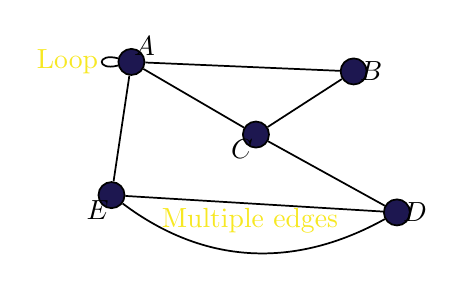
\begin{tikzpicture}[scale=0.5]
[every node/.style={inner sep=0pt}]
\node (1) [circle, minimum size=6pt, fill=cc, line width=0.625pt, draw=black] at (114.375pt, -155.0pt)  {};
\node (2) [circle, minimum size=6pt, fill=cc, line width=0.625pt, draw=black] at (275.0pt, -161.875pt)  {};
\node (3) [circle, minimum size=6pt, fill=cc, line width=0.625pt, draw=black] at (204.375pt, -207.5pt)  {};
\node (4) [circle, minimum size=6pt, fill=cc, line width=0.625pt, draw=black] at (100.0pt, -251.25pt)  {};
\node (5) [circle, minimum size=6pt, fill=cc, line width=0.625pt, draw=black] at (306.25pt, -263.75pt)  {};
\draw [line width=0.625, color=black] (1) to  (2);
\draw [line width=0.625, color=black] (1) to  (3);
\draw [line width=0.625, color=black] (3) to  (2);
\draw [line width=0.625, color=black] (5) to  (3);
\draw [line width=0.625, color=black] (5) to  (4);
\draw [line width=0.625, color=black] (4) to  [in=209, out=323] (5);
\node [color=aa] at (200pt,-270pt) {Multiple edges};
\draw [line width=0.625, color=black] (1) to  (4);
\draw [line width=0.625, color=black, loop left] (1) to (1);
\node[xshift=-0.3cm,left,color=aa] at (1) {Loop};
\node at (123.75pt, -143.75pt) {\textcolor{black}{$A$}};
\node at (287.5pt, -161.875pt) {\textcolor{black}{$B$}};
\node at (194.375pt, -218.125pt) {\textcolor{black}{$C$}};
\node at (90.0pt, -261.875pt) {\textcolor{black}{$E$}};
\node at (319.375pt, -263.75pt) {\textcolor{black}{$D$}};
\end{tikzpicture}
\end{center}

\begin{alertblock}{Simple Graph}
	A \textbf{Simple Graph} has no loops nor multiple edges. 
\end{alertblock}
A simple graph will thus have only 1s in its adjacency matrix.

\end{frame}

\begin{frame}{Connected and Complete Graphs}
	\begin{alertblock}{Connected}
		A graph is \textbf{connected} if any vertex can be reached via the edges from any other vertex.  
		
	\end{alertblock}
	\begin{alertblock}{Complete}
		A graph is \textbf{complete} if there is an edge between every pair of vertices. We denote this $K_n$ where  $n$ is the number of vertices. The adjacency matrix will be the matrix of ones minus the identity.

		It will have  $^n C _ 2 = n\frac{n-1}{2}$ edges.
		
	\end{alertblock}
\end{frame}

\begin{frame}{Graph Complements}
	\begin{alertblock}{Complement}
		The \textbf{complement} of a graph $G$, denoted  $G'$, is the graph with same vertex set but where all the non-edges of  $G$ become edges of  $G'$ and all the edges of  $G$ become non-edges of  $G'$. 

		Its adjacency matrix is equal to that of the correctly sized complete graph subtract the matrix of  $G$.
	\end{alertblock}

	Taking the union of all the edges will necessarily give you the entire complete graph.

\begin{center}
	\usetikzlibrary{shapes.geometric}
	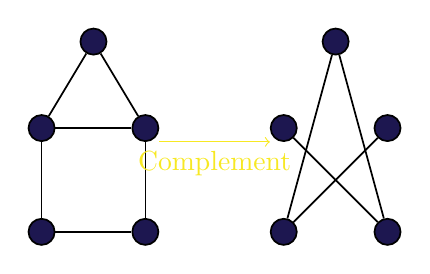
\begin{tikzpicture}[scale=0.5]
[every node/.style={inner sep=0pt}]
\node (1) [circle, minimum size=6pt, fill=cc, line width=0.625pt, draw=black] at (125.0pt, -250.0pt)  {};
\node (2) [circle, minimum size=6pt, fill=cc, line width=0.625pt, draw=black] at (125.0pt, -175.0pt)  {};
\node (3) [circle, minimum size=6pt, fill=cc, line width=0.625pt, draw=black] at (162.5pt, -112.5pt)  {};
\node (4) [circle, minimum size=6pt, fill=cc, line width=0.625pt, draw=black] at (200.0pt, -175.0pt)  {};
\node (5) [circle, minimum size=6pt, fill=cc, line width=0.625pt, draw=black] at (200.0pt, -250.0pt)  {};
\node (6) [circle, minimum size=6pt, fill=cc, line width=0.625pt, draw=black] at (300.0pt, -250.0pt)  {};
\node (7) [circle, minimum size=6pt, fill=cc, line width=0.625pt, draw=black] at (300.0pt, -175.0pt)  {};
\node (8) [circle, minimum size=6pt, fill=cc, line width=0.625pt, draw=black] at (337.5pt, -112.5pt)  {};
\node (9) [circle, minimum size=6pt, fill=cc, line width=0.625pt, draw=black] at (375.0pt, -175.0pt)  {};
\node (10) [circle, minimum size=6pt, fill=cc, line width=0.625pt, draw=black] at (375.0pt, -250.0pt)  {};
\draw [line width=0.625, color=black] (2) to  (1);
\draw [line width=0.625, color=black] (3) to  (2);
\draw [line width=0.625, color=black] (3) to  (4);
\draw [line width=0.625, color=black] (4) to  (5);
\draw [line width=0.625, color=black] (2) to  (4);
\draw [line width=0.625, color=black] (1) to  (5);
\draw [line width=0.625, color=black] (6) to  (8);
\draw [line width=0.625, color=black] (8) to  (10);
\draw [line width=0.625, color=black] (9) to  (6);
\draw [line width=0.625, color=black] (7) to  (10);
\draw [color=aa,->] (210pt,-185pt) -- (290pt,-185pt) node [midway,below] {Complement};
\end{tikzpicture}
	
\end{center}
	
\end{frame}

\begin{frame}{Bipartite Graphs}
	\begin{alertblock}{Bipartite Graph}
		A \textbf{bipartite graph} can have its vertices subdivided into two distinct subsets such that all the edges in the graph go from one subgroup to the other. 
	\end{alertblock}
	\begin{center}
		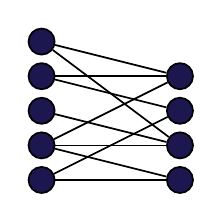
\begin{tikzpicture}[scale=0.5]
[every node/.style={inner sep=0pt}]
\node (1) [circle, minimum size=6pt, fill=cc, line width=0.625pt, draw=black] at (100.0pt, -250.0pt)  {};
\node (2) [circle, minimum size=6pt, fill=cc, line width=0.625pt, draw=black] at (100.0pt, -225.0pt)  {};
\node (3) [circle, minimum size=6pt, fill=cc, line width=0.625pt, draw=black] at (100.0pt, -200.0pt)  {};
\node (4) [circle, minimum size=6pt, fill=cc, line width=0.625pt, draw=black] at (100.0pt, -175.0pt)  {};
\node (5) [circle, minimum size=6pt, fill=cc, line width=0.625pt, draw=black] at (100.0pt, -150.0pt)  {};
\node (6) [circle, minimum size=6pt, fill=cc, line width=0.625pt, draw=black] at (200.0pt, -250.0pt)  {};
\node (7) [circle, minimum size=6pt, fill=cc, line width=0.625pt, draw=black] at (200.0pt, -225.0pt)  {};
\node (8) [circle, minimum size=6pt, fill=cc, line width=0.625pt, draw=black] at (200.0pt, -200.0pt)  {};
\node (9) [circle, minimum size=6pt, fill=cc, line width=0.625pt, draw=black] at (200.0pt, -175.0pt)  {};
\draw [line width=0.625, color=black] (5) to  (9);
\draw [line width=0.625, color=black] (4) to  (9);
\draw [line width=0.625, color=black] (3) to  (7);
\draw [line width=0.625, color=black] (2) to  (7);
\draw [line width=0.625, color=black] (1) to  (6);
\draw [line width=0.625, color=black] (5) to  (7);
\draw [line width=0.625, color=black] (4) to  (8);
\draw [line width=0.625, color=black] (9) to  (2);
\draw [line width=0.625, color=black] (6) to  (2);
\draw [line width=0.625, color=black] (8) to  (1);
\end{tikzpicture}
\end{center}

\begin{alertblock}{Complete Bipartite Graph}
	A \textbf{complete bipartite graph} is a bipartite graph with all the possible edges from one subset to the other. It is denoted $K_{m,n}$ where $m$ and  $n$ are the size of the two subsets. 
\end{alertblock}
	\begin{center}
		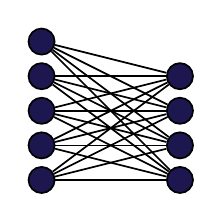
\begin{tikzpicture}[scale=0.5]
[every node/.style={inner sep=0pt}]
\node (1) [circle, minimum size=6pt, fill=cc, line width=0.625pt, draw=black] at (100.0pt, -250.0pt)  {};
\node (2) [circle, minimum size=6pt, fill=cc, line width=0.625pt, draw=black] at (100.0pt, -225.0pt)  {};
\node (3) [circle, minimum size=6pt, fill=cc, line width=0.625pt, draw=black] at (100.0pt, -200.0pt)  {};
\node (4) [circle, minimum size=6pt, fill=cc, line width=0.625pt, draw=black] at (100.0pt, -175.0pt)  {};
\node (5) [circle, minimum size=6pt, fill=cc, line width=0.625pt, draw=black] at (100.0pt, -150.0pt)  {};
\node (6) [circle, minimum size=6pt, fill=cc, line width=0.625pt, draw=black] at (200.0pt, -250.0pt)  {};
\node (7) [circle, minimum size=6pt, fill=cc, line width=0.625pt, draw=black] at (200.0pt, -225.0pt)  {};
\node (8) [circle, minimum size=6pt, fill=cc, line width=0.625pt, draw=black] at (200.0pt, -200.0pt)  {};
\node (9) [circle, minimum size=6pt, fill=cc, line width=0.625pt, draw=black] at (200.0pt, -175.0pt)  {};
\draw [line width=0.625, color=black] (1) to  (9);
\draw [line width=0.625, color=black] (1) to  (8);
\draw [line width=0.625, color=black] (1) to  (7);
\draw [line width=0.625, color=black] (1) to  (6);
\draw [line width=0.625, color=black] (2) to  (9);
\draw [line width=0.625, color=black] (2) to  (8);
\draw [line width=0.625, color=black] (2) to  (7);
\draw [line width=0.625, color=black] (2) to  (6);
\draw [line width=0.625, color=black] (3) to  (9);
\draw [line width=0.625, color=black] (3) to  (8);
\draw [line width=0.625, color=black] (3) to  (7);
\draw [line width=0.625, color=black] (3) to  (6);
\draw [line width=0.625, color=black] (4) to  (9);
\draw [line width=0.625, color=black] (4) to  (8);
\draw [line width=0.625, color=black] (4) to  (7);
\draw [line width=0.625, color=black] (4) to  (6);
\draw [line width=0.625, color=black] (5) to  (9);
\draw [line width=0.625, color=black] (5) to  (8);
\draw [line width=0.625, color=black] (5) to  (7);
\draw [line width=0.625, color=black] (5) to  (6);
\end{tikzpicture} 


Above is $K_{5,4}$.
\end{center}
\end{frame}

\section{More graph properties}

\begin{frame}{Trails, Circuits and Cycles}
	\begin{alertblock}{Trail}
		A \textbf{trail} is a sequence of edges in which the end of edge (except for the last) is the beginning  of the next, and no edge is repeated. Vertex can be repeated though.
	\end{alertblock}
	\begin{center}
	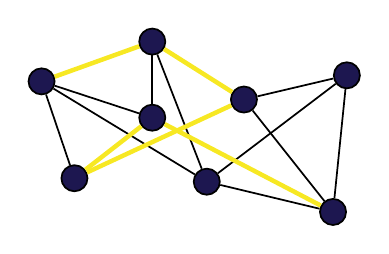
\begin{tikzpicture}[scale=0.5]
[every node/.style={inner sep=0pt}]
\node (1) [circle, minimum size=6pt, fill=cc, line width=0.625pt, draw=black] at (84.375pt, -185.0pt)  {};
\node (2) [circle, minimum size=6pt, fill=cc, line width=0.625pt, draw=black] at (164.375pt, -156.25pt)  {};
\node (3) [circle, minimum size=6pt, fill=cc, line width=0.625pt, draw=black] at (230.625pt, -198.125pt)  {};
\node (4) [circle, minimum size=6pt, fill=cc, line width=0.625pt, draw=black] at (305.0pt, -180.625pt)  {};
\node (5) [circle, minimum size=6pt, fill=cc, line width=0.625pt, draw=black] at (295.0pt, -279.375pt)  {};
\node (6) [circle, minimum size=6pt, fill=cc, line width=0.625pt, draw=black] at (203.75pt, -257.5pt)  {};
\node (7) [circle, minimum size=6pt, fill=cc, line width=0.625pt, draw=black] at (164.375pt, -211.25pt)  {};
\node (8) [circle, minimum size=6pt, fill=cc, line width=0.625pt, draw=black] at (108.125pt, -255.0pt)  {};
\draw [line width=1.625, color=aa] (1) to  (2);
\draw [line width=0.625, color=black] (1) to  (7);
\draw [line width=0.625, color=black] (1) to  (8);
\draw [line width=0.625, color=black] (1) to  (6);
\draw [line width=0.625, color=black] (2) to  (7);
\draw [line width=1.625, color=aa] (2) to  (3);
\draw [line width=0.625, color=black] (2) to  (6);
\draw [line width=0.625, color=black] (3) to  (4);
\draw [line width=1.625, color=aa] (3) to  (8);
\draw [line width=0.625, color=black] (3) to  (5);
\draw [line width=0.625, color=black] (4) to  (6);
\draw [line width=0.625, color=black] (4) to  (5);
\draw [line width=0.625, color=black] (5) to  (6);
\draw [line width=1.625, color=aa] (5) to  (7);
\draw [line width=1.625, color=aa] (7) to  (8);
\end{tikzpicture}
\end{center}

\begin{alertblock}{Circuit}
	A \textbf{circuit} is a closed trail, i.e. the end of the last edge is the start of the first. 
\end{alertblock}

	\begin{center}
	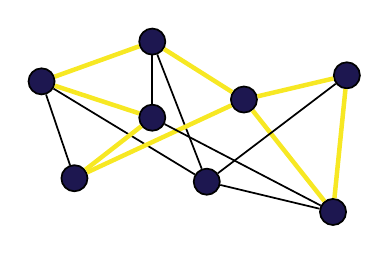
\begin{tikzpicture}[scale=0.5]
[every node/.style={inner sep=0pt}]
\node (1) [circle, minimum size=6pt, fill=cc, line width=0.625pt, draw=black] at (84.375pt, -185.0pt)  {};
\node (2) [circle, minimum size=6pt, fill=cc, line width=0.625pt, draw=black] at (164.375pt, -156.25pt)  {};
\node (3) [circle, minimum size=6pt, fill=cc, line width=0.625pt, draw=black] at (230.625pt, -198.125pt)  {};
\node (4) [circle, minimum size=6pt, fill=cc, line width=0.625pt, draw=black] at (305.0pt, -180.625pt)  {};
\node (5) [circle, minimum size=6pt, fill=cc, line width=0.625pt, draw=black] at (295.0pt, -279.375pt)  {};
\node (6) [circle, minimum size=6pt, fill=cc, line width=0.625pt, draw=black] at (203.75pt, -257.5pt)  {};
\node (7) [circle, minimum size=6pt, fill=cc, line width=0.625pt, draw=black] at (164.375pt, -211.25pt)  {};
\node (8) [circle, minimum size=6pt, fill=cc, line width=0.625pt, draw=black] at (108.125pt, -255.0pt)  {};
\draw [line width=1.625, color=aa] (1) to  (2);
\draw [line width=1.625, color=aa] (1) to  (7);
\draw [line width=0.625, color=black] (1) to  (8);
\draw [line width=0.625, color=black] (1) to  (6);
\draw [line width=0.625, color=black] (2) to  (7);
\draw [line width=1.625, color=aa] (2) to  (3);
\draw [line width=0.625, color=black] (2) to  (6);
\draw [line width=1.625, color=aa] (3) to  (4);
\draw [line width=1.625, color=aa] (3) to  (8);
\draw [line width=1.625, color=aa] (3) to  (5);
\draw [line width=0.625, color=black] (4) to  (6);
\draw [line width=1.625, color=aa] (4) to  (5);
\draw [line width=0.625, color=black] (5) to  (6);
\draw [line width=0.625, color=black] (5) to  (7);
\draw [line width=1.625, color=aa] (7) to  (8);
\end{tikzpicture}
\end{center}

\begin{alertblock}{Cycle}
	A \textbf{cycle} is a circuit in which no vertex is repeated. 
\end{alertblock}
	\begin{center}
	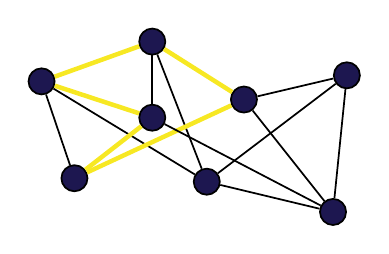
\begin{tikzpicture}[scale=0.5]
[every node/.style={inner sep=0pt}]
\node (1) [circle, minimum size=6pt, fill=cc, line width=0.625pt, draw=black] at (84.375pt, -185.0pt)  {};
\node (2) [circle, minimum size=6pt, fill=cc, line width=0.625pt, draw=black] at (164.375pt, -156.25pt)  {};
\node (3) [circle, minimum size=6pt, fill=cc, line width=0.625pt, draw=black] at (230.625pt, -198.125pt)  {};
\node (4) [circle, minimum size=6pt, fill=cc, line width=0.625pt, draw=black] at (305.0pt, -180.625pt)  {};
\node (5) [circle, minimum size=6pt, fill=cc, line width=0.625pt, draw=black] at (295.0pt, -279.375pt)  {};
\node (6) [circle, minimum size=6pt, fill=cc, line width=0.625pt, draw=black] at (203.75pt, -257.5pt)  {};
\node (7) [circle, minimum size=6pt, fill=cc, line width=0.625pt, draw=black] at (164.375pt, -211.25pt)  {};
\node (8) [circle, minimum size=6pt, fill=cc, line width=0.625pt, draw=black] at (108.125pt, -255.0pt)  {};
\draw [line width=1.625, color=aa] (1) to  (2);
\draw [line width=1.625, color=aa] (1) to  (7);
\draw [line width=0.625, color=black] (1) to  (8);
\draw [line width=0.625, color=black] (1) to  (6);
\draw [line width=0.625, color=black] (2) to  (7);
\draw [line width=1.625, color=aa] (2) to  (3);
\draw [line width=0.625, color=black] (2) to  (6);
\draw [line width=0.625, color=black] (3) to  (4);
\draw [line width=1.625, color=aa] (3) to  (8);
\draw [line width=0.625, color=black] (3) to  (5);
\draw [line width=0.625, color=black] (4) to  (6);
\draw [line width=0.625, color=black] (4) to  (5);
\draw [line width=0.625, color=black] (5) to  (6);
\draw [line width=0.625, color=black] (5) to  (7);
\draw [line width=1.625, color=aa] (7) to  (8);
\end{tikzpicture}
\end{center}
\end{frame}

\section{More Graph types}

\begin{frame}{Tree} 
	\begin{alertblock}{Tree}
		\begin{itemize}
			\item A \textbf{tree} is a simple and connected graph with no cycles.  
			\item A tree with $n$ vertices will have  $n-1$ edges.
			\item There is only one path between any pair of vertices in a tree.
		\end{itemize}
	\end{alertblock}
	\begin{center}
		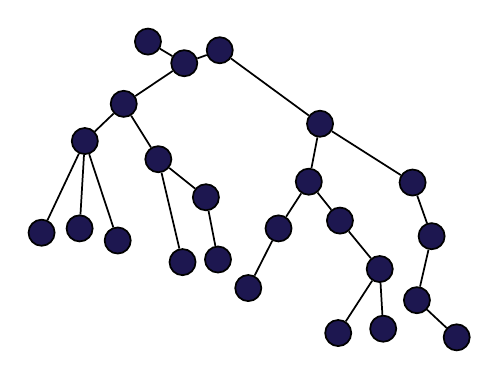
\begin{tikzpicture}[scale=0.5]
[every node/.style={inner sep=0pt}]
\node (1) [circle, minimum size=6pt, fill=cc, line width=0.625pt, draw=black] at (122.5pt, -98.75pt)  {};
\node (2) [circle, minimum size=6pt, fill=cc, line width=0.625pt, draw=black] at (148.75pt, -114.375pt)  {};
\node (3) [circle, minimum size=6pt, fill=cc, line width=0.625pt, draw=black] at (174.375pt, -105.0pt)  {};
\node (4) [circle, minimum size=6pt, fill=cc, line width=0.625pt, draw=black] at (105.0pt, -143.75pt)  {};
\node (5) [circle, minimum size=6pt, fill=cc, line width=0.625pt, draw=black] at (76.875pt, -170.625pt)  {};
\node (6) [circle, minimum size=6pt, fill=cc, line width=0.625pt, draw=black] at (130.0pt, -183.75pt)  {};
\node (7) [circle, minimum size=6pt, fill=cc, line width=0.625pt, draw=black] at (45.625pt, -236.875pt)  {};
\node (8) [circle, minimum size=6pt, fill=cc, line width=0.625pt, draw=black] at (73.125pt, -233.75pt)  {};
\node (9) [circle, minimum size=6pt, fill=cc, line width=0.625pt, draw=black] at (100.625pt, -242.5pt)  {};
\node (10) [circle, minimum size=6pt, fill=cc, line width=0.625pt, draw=black] at (164.375pt, -211.25pt)  {};
\node (11) [circle, minimum size=6pt, fill=cc, line width=0.625pt, draw=black] at (147.5pt, -258.125pt)  {};
\node (12) [circle, minimum size=6pt, fill=cc, line width=0.625pt, draw=black] at (173.125pt, -256.25pt)  {};
\node (13) [circle, minimum size=6pt, fill=cc, line width=0.625pt, draw=black] at (195.0pt, -276.875pt)  {};
\node (14) [circle, minimum size=6pt, fill=cc, line width=0.625pt, draw=black] at (246.875pt, -158.125pt)  {};
\node (15) [circle, minimum size=6pt, fill=cc, line width=0.625pt, draw=black] at (238.75pt, -200.0pt)  {};
\node (16) [circle, minimum size=6pt, fill=cc, line width=0.625pt, draw=black] at (261.25pt, -228.125pt)  {};
\node (17) [circle, minimum size=6pt, fill=cc, line width=0.625pt, draw=black] at (216.875pt, -233.75pt)  {};
\node (18) [circle, minimum size=6pt, fill=cc, line width=0.625pt, draw=black] at (313.75pt, -200.625pt)  {};
\node (19) [circle, minimum size=6pt, fill=cc, line width=0.625pt, draw=black] at (290.0pt, -263.125pt)  {};
\node (20) [circle, minimum size=6pt, fill=cc, line width=0.625pt, draw=black] at (260.0pt, -309.375pt)  {};
\node (21) [circle, minimum size=6pt, fill=cc, line width=0.625pt, draw=black] at (292.5pt, -306.25pt)  {};
\node (22) [circle, minimum size=6pt, fill=cc, line width=0.625pt, draw=black] at (327.5pt, -239.375pt)  {};
\node (23) [circle, minimum size=6pt, fill=cc, line width=0.625pt, draw=black] at (316.875pt, -285.625pt)  {};
\node (24) [circle, minimum size=6pt, fill=cc, line width=0.625pt, draw=black] at (345.625pt, -312.5pt)  {};
\draw [line width=0.625, color=black] (1) to  (2);
\draw [line width=0.625, color=black] (2) to  (3);
\draw [line width=0.625, color=black] (2) to  (4);
\draw [line width=0.625, color=black] (4) to  (5);
\draw [line width=0.625, color=black] (5) to  (7);
\draw [line width=0.625, color=black] (5) to  (8);
\draw [line width=0.625, color=black] (5) to  (9);
\draw [line width=0.625, color=black] (4) to  (6);
\draw [line width=0.625, color=black] (6) to  (11);
\draw [line width=0.625, color=black] (6) to  (10);
\draw [line width=0.625, color=black] (10) to  (12);
\draw [line width=0.625, color=black] (3) to  (14);
\draw [line width=0.625, color=black] (14) to  (15);
\draw [line width=0.625, color=black] (15) to  (17);
\draw [line width=0.625, color=black] (17) to  (13);
\draw [line width=0.625, color=black] (15) to  (16);
\draw [line width=0.625, color=black] (14) to  (18);
\draw [line width=0.625, color=black] (18) to  (22);
\draw [line width=0.625, color=black] (16) to  (19);
\draw [line width=0.625, color=black] (19) to  (20);
\draw [line width=0.625, color=black] (19) to  (21);
\draw [line width=0.625, color=black] (22) to  (23);
\draw [line width=0.625, color=black] (23) to  (24);
\end{tikzpicture}
\end{center}
\end{frame}

\begin{frame}[allowframebreaks]{Bridges of K\"onigsberg} 
	In 1736, the mathematician Leonhard Euler was asked whether it was possible to take a walk in the town of K\"onigsberg while crossing each bridge exactly once.

	In order to solve this he came up with the concept of an Eulerian graph.

	\begin{alertblock}{Eulerian}
		A graph is \textbf{Eulerian} if the whole graph is a circuit. 

	A graph is Eulerian $\equiv$ Every vertex has even degree.
		
	\end{alertblock}
	\begin{center}
		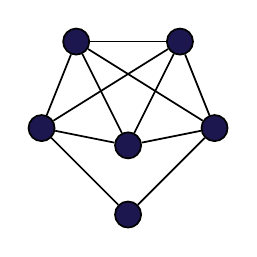
\begin{tikzpicture}[scale=0.5]
[every node/.style={inner sep=0pt}]
\node (1) [circle, minimum size=6pt, fill=cc, line width=0.625pt, draw=black] at (125.0pt, -175.0pt)  {};
\node (2) [circle, minimum size=6pt, fill=cc, line width=0.625pt, draw=black] at (200.0pt, -175.0pt)  {};
\node (3) [circle, minimum size=6pt, fill=cc, line width=0.625pt, draw=black] at (100.0pt, -237.5pt)  {};
\node (6) [circle, minimum size=6pt, fill=cc, line width=0.625pt, draw=black] at (162.5pt, -250.0pt)  {};
\node (5) [circle, minimum size=6pt, fill=cc, line width=0.625pt, draw=black] at (225.0pt, -237.5pt)  {};
\node (4) [circle, minimum size=6pt, fill=cc, line width=0.625pt, draw=black] at (162.5pt, -300.0pt)  {};
\draw [line width=0.625, color=black] (1) to  (2);
\draw [line width=0.625, color=black] (1) to  (6);
\draw [line width=0.625, color=black] (2) to  (6);
\draw [line width=0.625, color=black] (2) to  (3);
\draw [line width=0.625, color=black] (1) to  (5);
\draw [line width=0.625, color=black] (1) to  (3);
\draw [line width=0.625, color=black] (2) to  (5);
\draw [line width=0.625, color=black] (3) to  (6);
\draw [line width=0.625, color=black] (6) to  (5);
\draw [line width=0.625, color=black] (4) to  (5);
\draw [line width=0.625, color=black] (3) to  (4);
\end{tikzpicture}
\end{center}

\begin{alertblock}{Semi-Eulerian}
	A graph is \textbf{Semi-Eulerian} if the whole graph is a trail. 
	A graph is Semi-Eulerian $\equiv$ Exactly two vertices have odd degree.
\end{alertblock}
	\begin{center}
		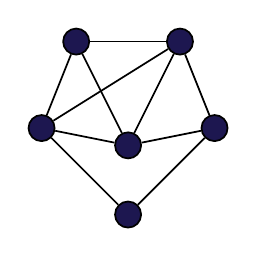
\begin{tikzpicture}[scale=0.5]
[every node/.style={inner sep=0pt}]
\node (1) [circle, minimum size=6pt, fill=cc, line width=0.625pt, draw=black] at (125.0pt, -175.0pt)  {};
\node (2) [circle, minimum size=6pt, fill=cc, line width=0.625pt, draw=black] at (200.0pt, -175.0pt)  {};
\node (3) [circle, minimum size=6pt, fill=cc, line width=0.625pt, draw=black] at (100.0pt, -237.5pt)  {};
\node (6) [circle, minimum size=6pt, fill=cc, line width=0.625pt, draw=black] at (162.5pt, -250.0pt)  {};
\node (5) [circle, minimum size=6pt, fill=cc, line width=0.625pt, draw=black] at (225.0pt, -237.5pt)  {};
\node (4) [circle, minimum size=6pt, fill=cc, line width=0.625pt, draw=black] at (162.5pt, -300.0pt)  {};
\draw [line width=0.625, color=black] (1) to  (2);
\draw [line width=0.625, color=black] (1) to  (6);
\draw [line width=0.625, color=black] (2) to  (6);
\draw [line width=0.625, color=black] (2) to  (3);
\draw [line width=0.625, color=black] (1) to  (3);
\draw [line width=0.625, color=black] (2) to  (5);
\draw [line width=0.625, color=black] (3) to  (6);
\draw [line width=0.625, color=black] (6) to  (5);
\draw [line width=0.625, color=black] (4) to  (5);
\draw [line width=0.625, color=black] (3) to  (4);
\end{tikzpicture}
\end{center}

\begin{Problem}{The bridge problem}
	The bridge problem can be reduced to the graph shown below. Since all four vertices are odd the graph is not even Semi-Eulerian, two extra bridges would have to be added for it to be Eulerian. 
\end{Problem}
\begin{center}
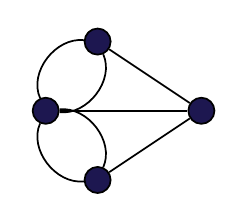
\begin{tikzpicture}[scale=0.5]
[every node/.style={inner sep=0pt}]
\node (1) [circle, minimum size=6pt, fill=cc, line width=0.625pt, draw=black] at (137.5pt, -237.5pt)  {};
\node (2) [circle, minimum size=6pt, fill=cc, line width=0.625pt, draw=black] at (250.0pt, -237.5pt)  {};
\node (3) [circle, minimum size=6pt, fill=cc, line width=0.625pt, draw=black] at (175.0pt, -187.5pt)  {};
\node (4) [circle, minimum size=6pt, fill=cc, line width=0.625pt, draw=black] at (175.0pt, -287.5pt)  {};
\draw [line width=0.625, color=black] (1) to  [in=174, out=114] (3);
\draw [line width=0.625, color=black] (1) to  [in=294, out=354] (3);
\draw [line width=0.625, color=black] (1) to  (2);
\draw [line width=0.625, color=black] (3) to  (2);
\draw [line width=0.625, color=black] (4) to  (2);
\draw [line width=0.625, color=black] (1) to  [in=66, out=6] (4);
\draw [line width=0.625, color=black] (4) to  [in=246, out=186] (1);
\end{tikzpicture}
\end{center}
\end{frame}
\begin{frame}{Hamiltonian Graphs}
	\begin{alertblock}{Hamiltonian cycle}
		A \textbf{Hamiltonian cycle} is a cycle which visits every vertex. Since a cycle is defined as a trail in which no vertex is repeated, a Hamiltonian cycle visits every vertex exactly once. 
	\end{alertblock}
	\begin{alertblock}{Hamiltonian Graph}
		A \textbf{Hamiltonian Graph} is one which \emph{contains} a Hamiltonian cycle. 

		We say contains as a Hamiltonian cycle will likely leave some edges unused despite using all the vertices.
	\end{alertblock}
	\begin{center}
		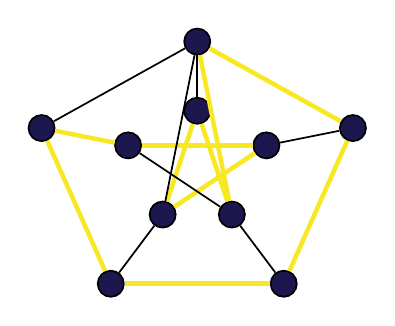
\begin{tikzpicture}[scale=0.5]
[every node/.style={inner sep=0pt}]
\node (1) [circle, minimum size=6pt, fill=cc, line width=0.625pt, draw=black] at (87.5pt, -200.0pt)  {};
\node (2) [circle, minimum size=6pt, fill=cc, line width=0.625pt, draw=black] at (312.5pt, -200.0pt)  {};
\node (4) [circle, minimum size=6pt, fill=cc, line width=0.625pt, draw=black] at (137.5pt, -312.5pt)  {};
\node (5) [circle, minimum size=6pt, fill=cc, line width=0.625pt, draw=black] at (262.5pt, -312.5pt)  {};
\node (3) [circle, minimum size=6pt, fill=cc, line width=0.625pt, draw=black] at (200.0pt, -137.5pt)  {};
\node (6) [circle, minimum size=6pt, fill=cc, line width=0.625pt, draw=black] at (200.0pt, -187.5pt)  {};
\node (7) [circle, minimum size=6pt, fill=cc, line width=0.625pt, draw=black] at (250.0pt, -212.5pt)  {};
\node (8) [circle, minimum size=6pt, fill=cc, line width=0.625pt, draw=black] at (225.0pt, -262.5pt)  {};
\node (9) [circle, minimum size=6pt, fill=cc, line width=0.625pt, draw=black] at (175.0pt, -262.5pt)  {};
\node (10) [circle, minimum size=6pt, fill=cc, line width=0.625pt, draw=black] at (150.0pt, -212.5pt)  {};
\draw [line width=1.625, color=aa] (7) to (9);
\draw [line width=1.625, color=aa] (9) to(6);
\draw [line width=1.625, color=aa] (6) to(8);
\draw [line width=1.625, color=aa] (8) to(3);
\draw [line width=1.625, color=aa] (3) to (2);
\draw [line width=1.625, color=aa] (2) to (5);
\draw [line width=1.625, color=aa] (5) to(4);
\draw [line width=1.625, color=aa] (4) to (1);
\draw [line width=1.625, color=aa] (1) to(10);
\draw [line width=1.625, color=aa] (10) to (7);
\draw [line width=0.625, color=black] (1) to (3);
\draw [line width=0.625, color=black] (3) to (6);
\draw [line width=0.625, color=black] (4) to (9);
\draw [line width=0.625, color=black] (5) to (8);
\draw [line width=0.625, color=black] (7) to (2);
\draw [line width=0.625, color=black] (3) to (9);
\draw [line width=0.625, color=black] (10) to (8);
\end{tikzpicture}
\end{center}
\end{frame}
\end{document}
